\section{Logische Gatter}
Die Komplexität einer Schaltung kann mit \textbf{Gatteräquivalents} $n_{ge}$ verglichen werden. \underline{1GE entsprechen 4 Transistoren}. Siehe \verweiseref{symbols}

\subsection{CMOS-Transistor}
Ein CMOS Transistor beinhaltet ein PMOS und ein NMOS Transistor. Dies hat folgende Vor/Nachteile:
\begin{itemize}[nosep]
	\pro kein statischer Stromverbrauch 
	\pro symmetrisches Schaltverhalten
	\pro hohe Störsicherheit
	\pro gebräuchlich und ideale Form für Integration
	\contra mehr Transistoren
\end{itemize}

\noindent
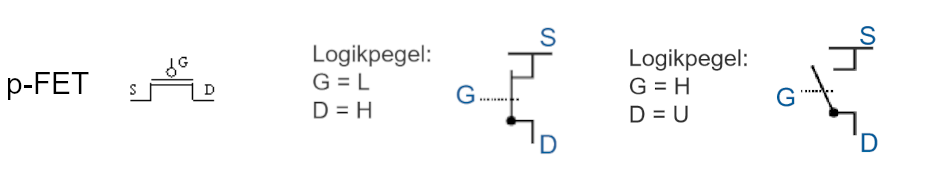
\includegraphics[width=\columnwidth]{./Images/p-fet.png}
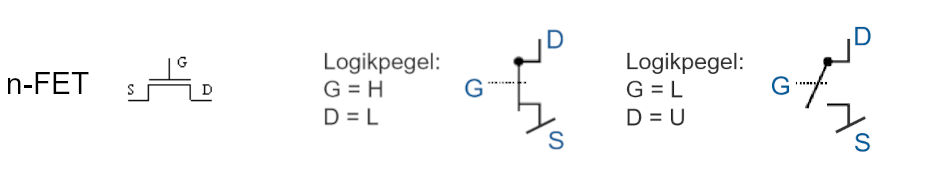
\includegraphics[width=\columnwidth]{./Images/n-fet.png}

\noindent
CMOS-Transistoren dürfen \textbf{NIE} direkt am Ausgang miteinander Verbunden werden (Kurzschluss von VDD nach GND)! Das Verbinden der Eingänge ist erlaubt.

\subsection{Eigenschaften}
\noindent\begin{minipage}{\textwidth}
	\noindent\textbf{Pegelbereich}

	\begin{minipage}{0.25\textwidth}
		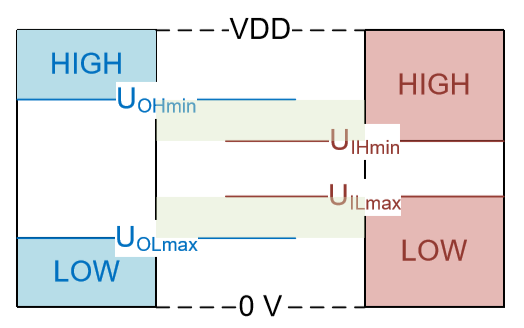
\includegraphics[width=0.8\linewidth,keepaspectratio=true]{./Images/Pegelbereich.png}
	\end{minipage}%%% to prevent a space
	\begin{minipage}{0.25\textwidth}

		\textbf{High-Pegel:}\\ $U_{nH} = U_{OHmin} - U_{IHmin}$ \\
		\textbf{Low-Pegel:}\\ $U_{nL} = U_{ILmax} - U_{OLmin}$
	\end{minipage}
\end{minipage}

\noindent\begin{minipage}{\textwidth}
	\noindent\textbf{Transition Time}
	
	\begin{minipage}{0.25\textwidth}
		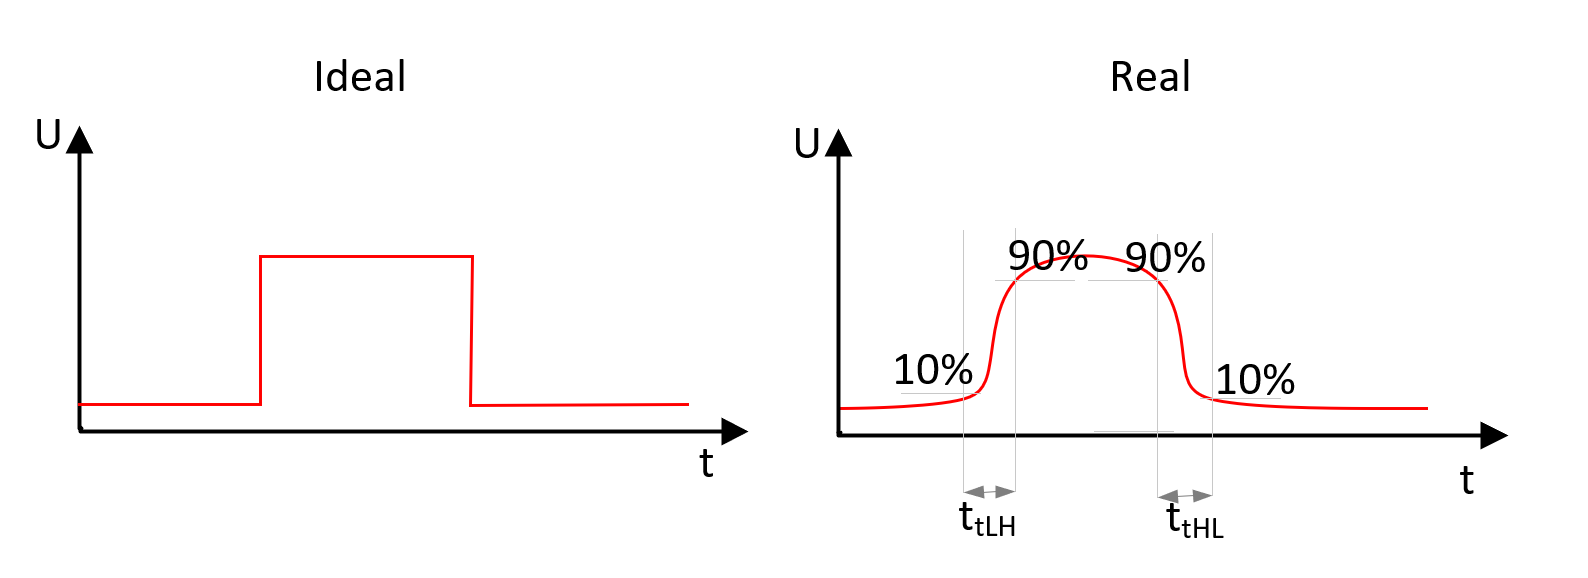
\includegraphics[width=\linewidth,keepaspectratio=true]{./Images/transitiontime.png}
	\end{minipage}%%% to prevent a space
	\begin{minipage}{0.2\textwidth}
		Zeit zwischen 10\% und 90\% von V$_\text{max}$\\
	\end{minipage}
\end{minipage}

\noindent\begin{minipage}{\textwidth}
	\noindent\textbf{Propagation Time}
	
	\begin{minipage}{0.25\textwidth}
		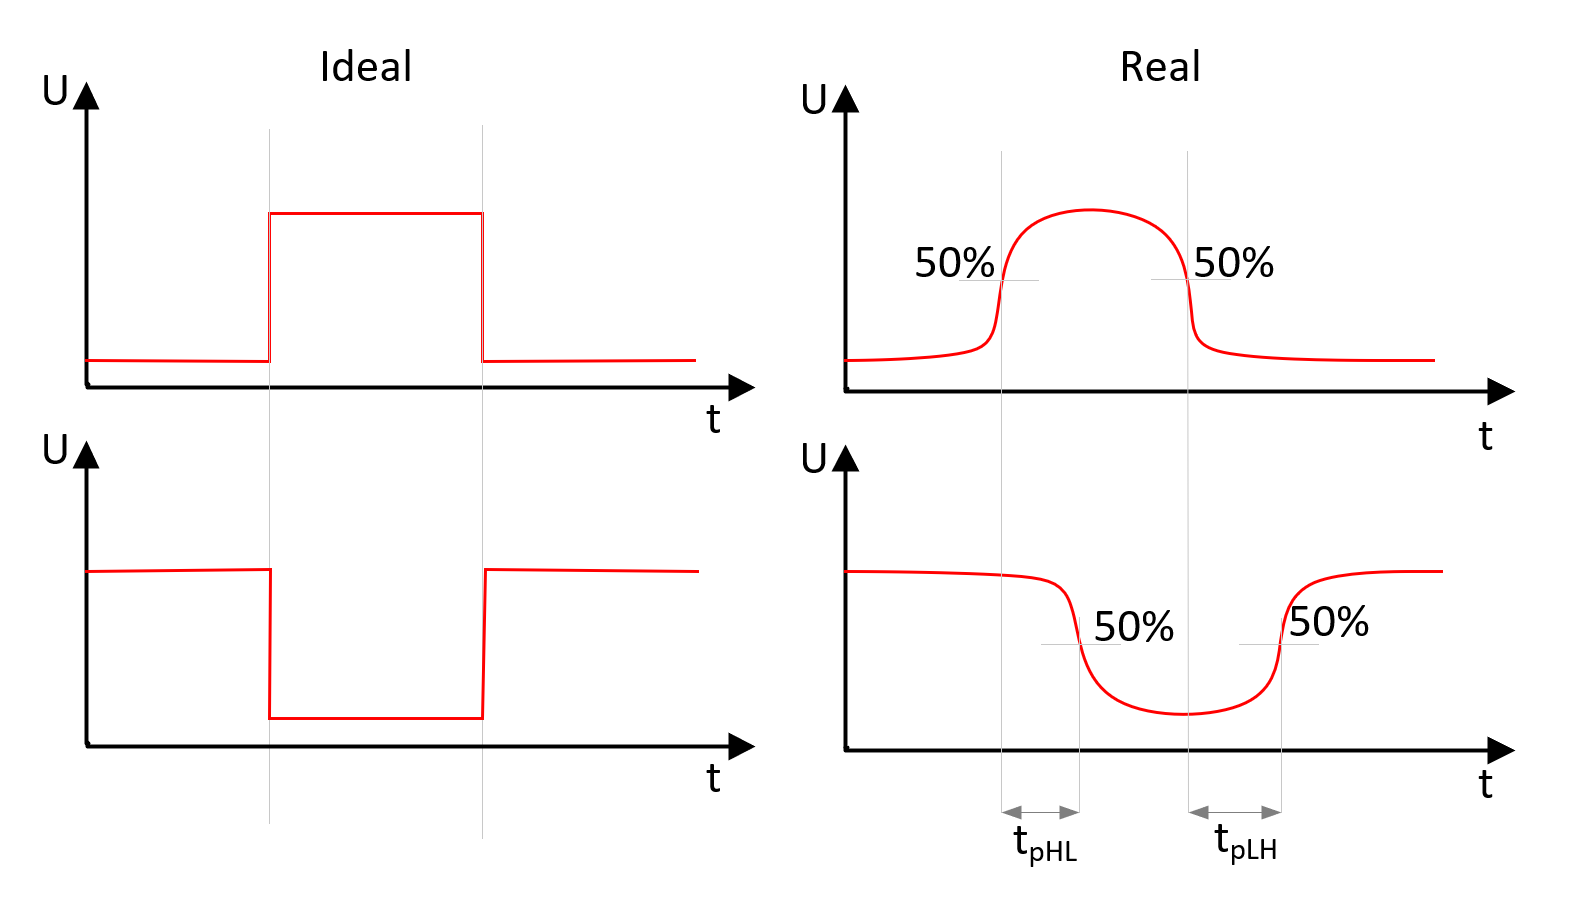
\includegraphics[width=\linewidth,keepaspectratio=true]{./Images/propagationtime.png}
	\end{minipage}%%% to prevent a space
	\begin{minipage}{0.20\textwidth}
		Zeit zwischen 50\% von V$_\text{max}$ Eingang und 50\% von  V$_\text{max}$ am Ausgang
	\end{minipage}
\end{minipage}


\noindent\begin{minipage}{\textwidth}
	\noindent\textbf{Propagation Time}
	
	\begin{minipage}{0.2\textwidth}
		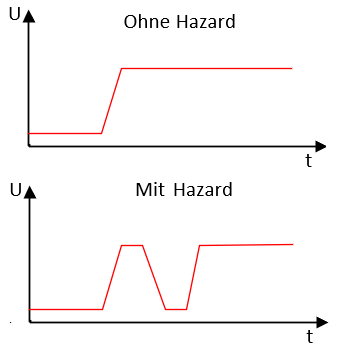
\includegraphics[width=\linewidth,keepaspectratio=true]{./Images/hazard.png}
	\end{minipage}%%% to prevent a space
	\begin{minipage}{0.25\textwidth}
			Bei \textbf{statischen}-Hazards ändert sich der Pegel einmalig, obwohl die Eingänge gleichbleibend sind. \textbf{Dynamische}-Hazards ändern Pegel mehrmalig.
	\end{minipage}
\end{minipage}

